%---------------------------------------------------
% Nombre: capitulo2.tex  
% 
% Texto del cap�tulo 2
%---------------------------------------------------

\chapter{Preprocesado}
\label{preprocesado}

En este cap�tulo enunciaremos el proceso de preprocesado llevado a cabo durante la realizaci�n de la pr�ctica. Cabe destacar, que por facilitar la comprensi�n todo el proceso se enuncia en este cap�tulo, pero hay ciertos puntos como el del proceso de undersampling (secci�n \ref{undersampling}) y el de corte de las im�genes  (secci�n \ref{cut}) que surgen fruto de cambios e ideas en el proceso de aprendizaje y entrenamiento de las redes neuronales. 

\section{Resize data}

Como veremos en el cap�tulo de conclusion, uno de los requisitos y mayores problemas que esta pr�ctica a ofrecido han sido las limitaciones de memoria tanto de principal para computo como de memoria secundaria para almacenar todas las im�genes y sus diferentes versiones. Con el fin de poder manejar estas m�s eficientemente se ha realizado un resize de las mismas a tama�o de 256x256px, para ello hemos seguido el siguiente script en R. 

\lstset{language=R, breaklines=true, basicstyle=\footnotesize}
\lstset{numbers=left, numberstyle=\tiny, stepnumber=1, numbersep=-2pt}
\begin{lstlisting}
  #-------------------------------------------------------------------------------

  # Clear workspace
  rm(list=ls())

  #-------------------------------------------------------------------------------
  # Load and pre-process images
  #-------------------------------------------------------------------------------

  # Set run parameters parameters
  test_img_path <- "."
  width  <- 256
  height <- 256


  #-------------------------------------------------------------------------------
  # Load and pre-process train images
  #-------------------------------------------------------------------------------

  # Load EBImage library
  library(EBImage)

  # Load images into a dataframe
  library(gsubfn)
  img_file_list <- list.files(path = test_img_path, pattern = "*.jpg", full.names = TRUE, recursive = TRUE)

  train_df <- data.frame()

  for(i in 1:length(img_file_list)) {
    img_file_name <- img_file_list[i]
    #img_class <- strapplyc(img_file_list[i], ".*/Type_(.*)/")[[1]]
    img <- readImage(img_file_name)
    img_resized <- resize(img, w=width, h=height)
    
    name <- paste("reducidas",img_file_name, sep="/")
    dir.create("reducidas", showWarnings = FALSE)
    writeImage(img_resized, name)
    
  }  
\end{lstlisting}

\section{Cut data}
\label{cut}


\section{Data Augmentation}

\lstset{language=R, breaklines=true, basicstyle=\footnotesize}
\lstset{numbers=left, numberstyle=\tiny, stepnumber=1, numbersep=-2pt}
\begin{lstlisting}
        
\end{lstlisting}



\section{Undersampling}
\label{undersampling}


%\begin{figure}[H]
%	\centering
%		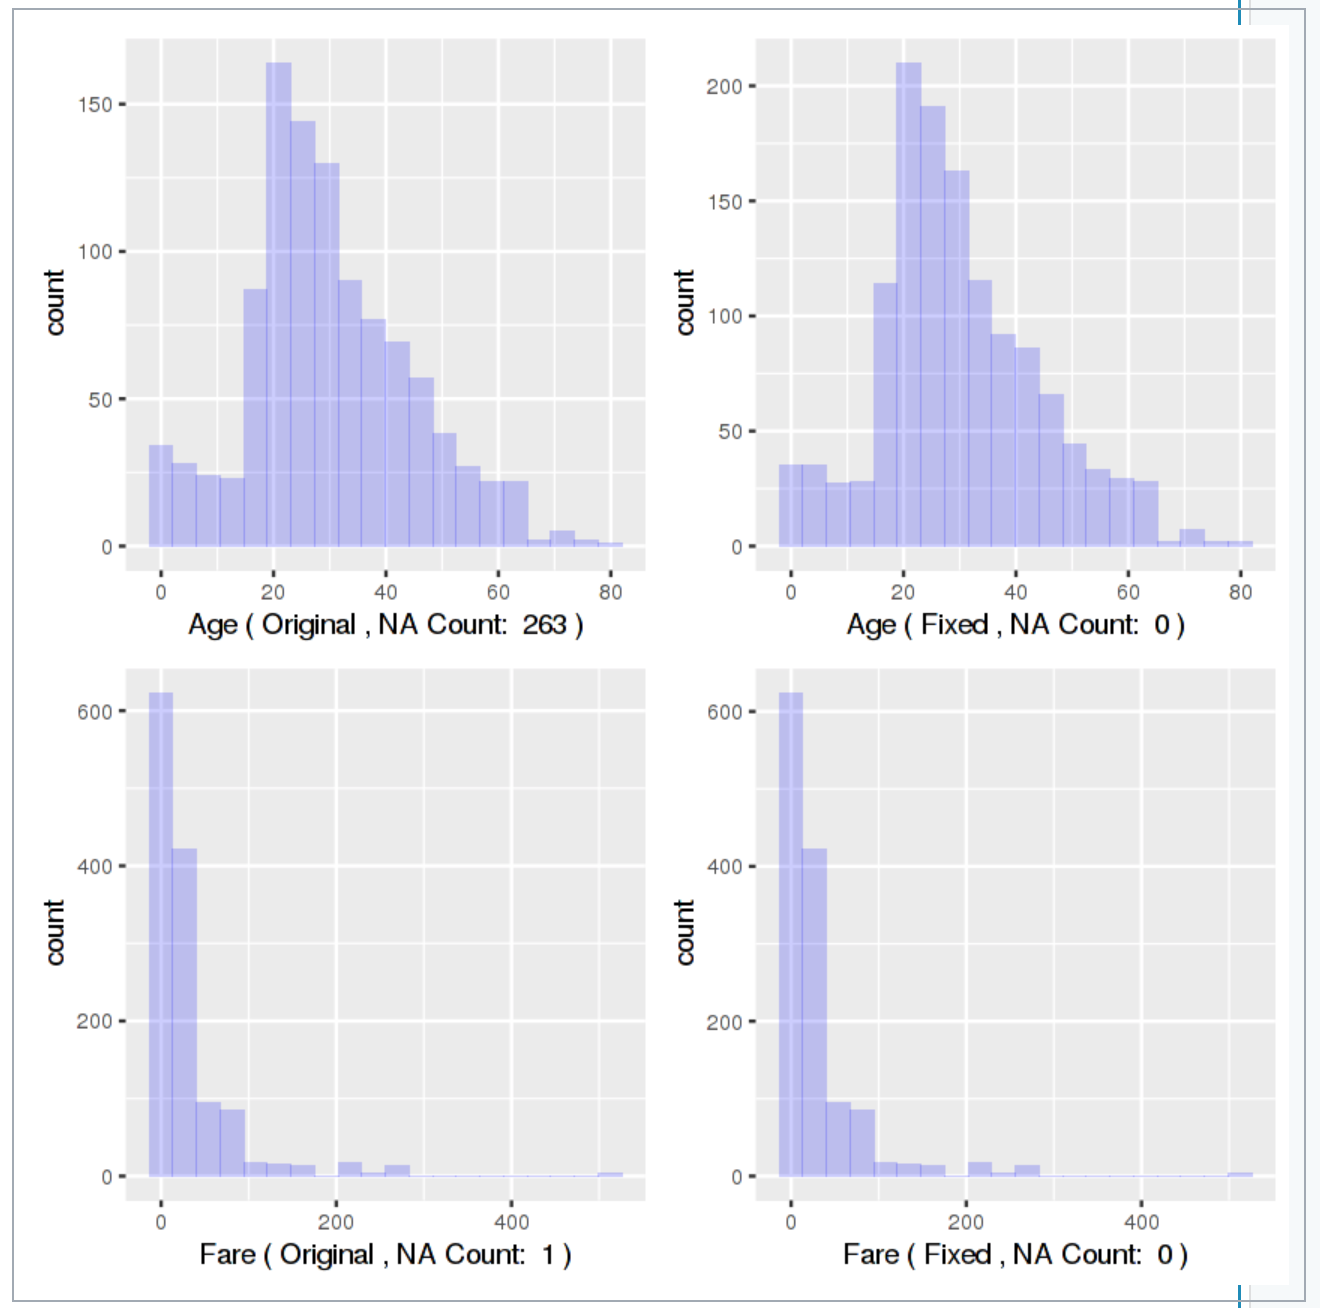
\includegraphics[scale=0.4]{./Capitulo2/imagenes/histcomp.png}
%		\caption{Comparaci�n de la imputaci�n de valores perdidos.}
%	\label{histcomp}
%\end{figure} 




\pagebreak
\clearpage
%---------------------------------------------------